\documentclass[11pt,oneside]{book}

\usepackage[T1]{fontenc}
\usepackage[french]{babel}

\usepackage[utf8]{inputenc}
\usepackage{graphicx}
\usepackage{grffile}
\usepackage{longtable}
\usepackage{wrapfig}
\usepackage{rotating}
\usepackage[normalem]{ulem}
\usepackage{amsmath}
\usepackage{textcomp}
\usepackage{amssymb}
\usepackage{capt-of}
\usepackage[colorlinks=true,linkcolor=black,citecolor=black]{hyperref}
\usepackage{textgreek}
\usepackage{minted}
\usepackage{framed}
\usepackage{mdframed}
\usepackage{geometry}
\usepackage{titlesec}
\usepackage{pdfpages}
\usepackage{fancyhdr}
\usepackage{colortbl}
\usepackage[dvipsnames]{xcolor}
\usepackage[textwidth=16mm]{todonotes}
\usepackage{color}

\newcommand{\as}[1]{\todo[color=green!40,size=\tiny,caption={}]{#1}}
\newcommand{\asi}[1]{\todo[inline,caption={},color=green!40]{#1}}

\newcommand{\hlink}[2]{\hyperlink{#1}{\color{magenta} #2}}

\geometry{
a4paper,
left=18mm,
right=18mm,
top=20mm,
bottom=20mm
}

\begin{document}


\includepdf[pages=-]{page1.pdf}

\pagestyle{empty}
\fontfamily{cmss}
\selectfont

\setlength{\parindent}{4mm}

\setcounter{tocdepth}{1}
\tableofcontents
\pagenumbering{gobble}

\chapter{Introduction}
\pagenumbering{arabic}
\setcounter{page}{1}
\pagestyle{fancy}
\fancyhf{}
\cfoot[\thepage]{\thepage}

Ce projet nous a été proposé par l’équipe \href{https://www-intuidoc.irisa.fr/}{IntuiDoc} de l’\href{https://www.irisa.fr/}{IRISA}, en étroite collaboration avec la startup \href{http://www.doptim.eu}{Doptim} et avec le soutien de Jean-Yves LE CLERC, conservateur du patrimoine aux \href{http://archives.ille-et-vilaine.fr/fr}{archives départementales} d'Ille-et-Vilaine. Tout au long de l’année, nous serons encadrés par Bertrand COÜASNON, enseignant-chercheur membre d'IntuiDoc, Erwan FOUCHÉ, chef de projet chez \href{https://www.soprasteria.com/fr}{Sopra Steria}, Julien BOUVET, ingénieur chez Sopra Steria également. Nous serons aussi accompagnés par Sophie TARDIVEL, responsable et \textit{data scientist} chez Doptim.

\paragraph{}
Dans ce rapport, nous rappellerons le contexte du projet qui justifie certains choix de conception. Nous décrirons ensuite l’architecture logicielle générale de notre projet ainsi que les diagrammes de séquences illustrant le fonctionnement interne de ce dernier. Puis, nous décrirons plus en détail les deux itérations prévues, la première répondant simplement au cahier des charges, la seconde complétant l'ensemble des fonctionnalités décrites dans le rapport de spécification, et donnant plus d'importance à l'ergonomie de la solution logicielle.

% ---


\chapter{Rappel du contexte}

\section{Les acteurs du projet}

Notre projet est encadré par Bertrand COÜASNON, enseignant à l’INSA de Rennes et membre de l’équipe de recherche IntuiDoc à l’IRISA, ainsi que Erwan Fouché et Julien Bouvet, ingénieurs au sein de l’entreprise Sopra Steria. Nous réalisons ce projet en relation avec Jean-Yves LE CLERC, conservateur et responsable de la numérisation  aux archives départementales d’Ille-et-Vilaine, et Sophie Tardivel, responsable et data scientist chez Doptim.

\paragraph{}

Notre équipe est composée de huit étudiants INSA, tous en quatrième année au département informatique : Enzo CRANCE, Kevin DESPOULAINS, Laure DU MESNILDOT, Valentin FOUCHER, Gaël GENDRON, Corentin GUILLOUX, Charlotte RICHARD et Timothée NEITTHOFFER.

\section{Le périmètre fonctionnel}

Ce projet nous a été proposé par Bertrand COÜASNON et a pour objectif de générer de manière automatique des bases d’apprentissage pour des reconnaisseurs d’écriture manuscrite et imprimée à partir de documents numérisés et de leur transcription numérique. Les reconnaisseurs d’écriture ont besoin d’apprendre à reconnaître les caractères manuscrits au travers d'exemples d'images dont on connaît le contenu. Notre but est donc de concevoir un logiciel et de le développer afin qu’il puisse générer ces exemples dans des bases d’apprentissage. Au travers d’une interface (IHM), l’utilisateur pourra également modifier les exemples générés dans la base afin de les corriger s’ils ont mal été générés. Il pourra également les supprimer de la base.

\paragraph{}

Ce projet s’installe dans la continuité des efforts de transformation numérique des archives. En effet, les modes de consommation de l’information changent et tendent à se diriger vers le tout numérique : c’est dans cette approche que les archives départementales d’Ille-et-Vilaine font appel à nos services afin de permettre à tous d’accéder aux informations archivées depuis chez soi via une application web, évitant ainsi de se déplacer dans les locaux des archives.

\section{Les éléments en entrée}

\subsection{Les données en entrée de l'application}

Les données en entrée de l’application sont les documents manuscrits ou imprimés numérisés, leur transcription et des annotations. Ces documents pourront être de différents types : des articles de presse, des actes de naturalisation ou de mariage, etc. Ces données devront être formatées correctement pour être utilisées par notre programme.

\newpage

\subsection{Les sources d'information existantes}

Tout au long du projet, nous pourrons nous aider d’une base existante contenant des documents numérisés ainsi que leur transcription et des annotations. Elle servira donc à tester notre programme lors de son développement. Un détecteur de lignes nous est également fourni par Bertrand COÜASNON.

\section{Le périmètre de qualification}

Le résultat attendu par le client est une application pouvant être utilisable par n’importe quelle personne disposant d’un reconnaisseur d’écriture manuscrite et désirant générer une base d’apprentissage rapidement à partir de documents déjà retranscrits. Le niveau de qualité attendu est donc assez élevé, il faudra privilégier la qualité des fonctionnalités plutôt que leur quantité. C’est pourquoi nous sommes partis sur un logiciel simple, fonctionnant sans aucune connexion internet. En plus des attentes fonctionnelles, la qualité du code doit également être soignée. Avoir un code propre, lisible et compréhensible est un point-clé, en effet cela permettra aux promotions suivantes de continuer le projet si toutes les fonctionnalités n’ont pas été implémentées, ou si de nouvelles idées d’amélioration émergent dans le futur.

\paragraph{}

Afin d’arriver à ce niveau de qualification, nous allons devoir mettre en place plusieurs  stratégies. Tout d’abord nous ferons des tests unitaires sur l’application afin de nous assurer de la robustesse du système de gestion des données. Ensuite, du côté client, les tests seront surtout faits directement sur l’interface utilisateur pour détecter des problèmes fonctionnels d’une part et des problèmes d’affichage d’autre part.

\section{Le calendrier}

Les ressources humaines ne seront pas les mêmes tout au long du projet. En effet certains membres du groupe partent en mobilité lors du second semestre de l’année : Kevin DESPOULAINS, Gaël GENDRON et Corentin GUILLOUX. Il restera donc cinq membres pour la partie développement de l’application. Tout au long de ce projet, des rapports seront à rédiger afin de rendre compte de l’évolution du projet, notamment des étapes clés de son élaboration.

\begin{center}

\begin{tabular}{ | l | l | }
	\hline
	\textbf{Livrables du projet} & \textbf{Date de rendu} \\
	\hline
	Rapport de pré-étude associé à la phase d'analyse & Jeudi 25 octobre 2018 \\
	\hline
	Rapport de spécification fonctionnelle  & Vendredi 30 novembre 2018 \\
	\hline
	Dossier de planification & Mardi 18 décembre 2018 \\
	\hline
	Rapport de conception logicielle & Vendredi 15 Février 2019 \\
	\hline
	Page HTML résumant le projet & Vendredi 29 mars 2019 \\
	\hline
	Rapport final  & Mardi 7 mai 2019 \\
	\hline
	Livraison du projet & Jeudi 9 mai 2019 \\
	\hline
\end{tabular}

\paragraph{}

\begin{tabular}{ | l | l | }
	\hline
	\textbf{Présentations du projet} & \textbf{Date} \\
	\hline
	Soutenance de planification  & Jeudi 20 décembre 2018 \\
	\hline
	Première soutenance de projet  & Vendredi 21 décembre 2018 \\
	\hline
	Dernière soutenance de projet & Jeudi 9 mai 2019 \\
	\hline
	Showroom des projets & Vendredi 10 mai 2019 \\
	\hline
\end{tabular}

\end{center}

\section{Analyse des risques}

Lors de la phase de développement de l’application, nous avons envisagé plusieurs risques potentiels qui pourraient retarder le bon déroulement du projet. Nous avons donc prévu dès maintenant des solutions, présentées ci-dessous, afin de pouvoir continuer à avancer normalement en cas de problème.

\paragraph{}

\noindent \textbf{Risque : } Absence non prévue (maladie, etc.)
\newline
\textbf{Impact : } Plus de travail pour les autres, nécessité de rattraper le retard pour l'absent
\newline
\textbf{Action 1 : } Prévenir au plus tôt dans la mesure du possible pour minimiser les effets de surprise
\newline
\textbf{Action 2 : } Bien commenter le code pour pouvoir reprendre facilement la partie de l’absent

\paragraph{}

\noindent \textbf{Risque : } Surcharge de travail avec les cours
\newline
\textbf{Impact : } Moins de temps pour travailler sur le projet
\newline
\textbf{Action : } Prendre de l’avance sur les périodes moins chargées

\paragraph{}

\noindent \textbf{Risque : } Bug incompréhensible, zone de blocage
\newline
\textbf{Impact : } Perte de temps et risque de retarder les autres membres de l’équipe
\newline
\textbf{Action : } En parler avec les autres pour ne pas rester coincé seul

\paragraph{}
 
\noindent \textbf{Risque : } Blocage dû à la parallélisation des tâches (exemple : le développeur de la partie
front-end en attente de la mise en place de la partie base de données)
\newline
\textbf{Impact : } Perte de temps et membres du groupe non utilisés
\newline
\textbf{Action : } Ne pas attendre en silence, en parler au chef de projet pour faire une autre tâche
en attendant

\paragraph{}

\noindent \textbf{Risque : } Problème relationnel entre des personnes du groupe
\newline
\textbf{Impact : } Création de conflits, perte de communication et donc d’informations
\newline
\textbf{Action 1 : } Mettre les choses à plat, ne pas faire monter les tensions en gardant le silence
\newline
\textbf{Action 2 : } En parler au chef d’équipe, qui sera chargé de désamorcer les tensions

\paragraph{}

\noindent \textbf{Risque : } Mauvaise interprétation de ce qui est demandé par le client
\newline
\textbf{Impact : } Perte de temps à développer inutilement
\newline
\textbf{Action : } Bien communiquer au sein du groupe et avec le client pour être sûr d’avoir la même vision des choses















% ---

\hypertarget{c6}{\chapter{Organisation du projet}}

\section{Méthodes de travail}

Cette année, nous avons décidé d’utiliser une méthode de travail suivant un cycle en V.
Cette méthode nous semble la plus adaptée pour notre cas. En effet, les limites du projet
sont clairement définies, de même que le cahier des charges et les spécifications générales.
Ainsi, durant la première phase du projet, au premier semestre, nous allons mettre en place
des réunions régulières pour bien évaluer le travail à réaliser. Durant la seconde phase,
au second semestre, nous effectuerons des réunions pour voir l’avancée de la programmation.

\paragraph{}
Comme le projet peut facilement être découpé en 4 parties (Préparation des données,
Base de données, IHM et Gestion du reconnaisseur), nous avons décidé de diviser notre
groupe en 4 pour pouvoir faire avancer le projet en parallèle. Nous estimons qu’il est
tout de même important de garder une forte communication et cohésion entre les différents
groupes, donc nous avons mis en place différents systèmes de communication. Pour gérer
l’organisation, nous utiliserons Trello et Microsoft Project. Pour le partage de fichiers,
notamment pour la rédaction des rapports, nous utiliserons Google Drive et Git.
Pour la gestion du code, nous utiliserons aussi Git. Enfin, pour communiquer, nous
utiliserons une conversation Messenger (qui servira à transmettre des informations de
manière rapide), un groupe Facebook (qui servira à publier la répartition des tâches et
les objectifs de chaque semaine de manière fixe et accessible) et probablement des salons
Discord qui permettront à chaque groupe de communiquer sans perturber les autres groupes.

\paragraph{}
Pour l’instant, nous avons décidé d’établir des réunions hebdomadaires (voire deux réunions
par semaine en cas de retard ou de livrables à rendre). Cette planification sera probablement
modifiée au second semestre lors du début du développement, car le groupe sera réduit de
moitié à cause des départs en mobilité. En effet, à partir du mois de janvier et du début du
second semestre, certaines personnes partiront faire une mobilité à l’étranger et ne
travailleront donc plus sur le projet. Notre groupe sera amputé de trois personnes : Kevin
DESPOULAINS, Gaël GENDRON et Corentin GUILLOUX.

\paragraph{}
L’arrivée ou le départ de membres n’est pas rare dans le déroulement d’un projet et nous avons
réfléchi à une organisation qui permet de faire une transition souple entre le premier semestre
où nous sommes huit et le second où nous serons cinq. Les membres partant à l’étranger ne
travailleront en effet pas seuls sur une partie mais leur travail sera réparti sur plusieurs
aspects du projet où ils travailleront avec des personnes restant au second semestre. Cette
répartition est faite pour qu’au moment de leur départ, il y ait au moins une personne du groupe
restant sachant exactement ce qui a été fait par les étudiants qui sont partis.

\section{Répartition des tâches}

Afin de répondre aux besoins du projet, nous avons mis en place 3 rôles. Ces 3 rôles ne sont pas fixes,
ils peuvent être modifiés en cas de besoin. Le premier rôle est le chef de projet. Ce rôle n’est donc pas
assigné de manière fixe, il change régulièrement. Nous avons établi un calendrier précis en figure 14
qui donne l’indication de qui est chef de projet à chaque instant.

\begin{mdframed}[frametitle={Figure 14 : Planning des rotations du rôle de chef de projet}, innerbottommargin=10]
\begin{center}
\begin{tabular}{ | l | l | l | }
\hline
{\textbf{Chef de projet}}   &   {\textbf{Début}}    &   {\textbf{Fin}}  \\ \hline \rowcolor[RGB]{182, 215, 168}
{Kevin DESPOULAINS}         &   {17/09/2018}        &	{07/10/2018}    \\ \hline \rowcolor[RGB]{255, 229, 153}
{Gaël GENDRON}              &   {08/10/2018}	    &	{28/10/2018}    \\ \hline \rowcolor[RGB]{249, 203, 156}
{Corentin GUILLOUX}         &   {05/11/2018}	    &	{30/11/2018}    \\ \hline \rowcolor[RGB]{234, 153, 153}
{Valentin FOUCHER}          &   {01/12/2018}	    &	{13/01/2019}    \\ \hline \rowcolor[RGB]{221, 126, 107}
{Enzo CRANCE}               &   {14/01/2019}	    &	{04/02/2019}    \\ \hline \rowcolor[RGB]{213, 166, 189}
{Charlotte RICHARD}         &   {05/02/2019}	    &	{10/03/2019}    \\ \hline \rowcolor[RGB]{180, 167, 214}
{Laure DU MESNILDOT}        &   {11/03/2019}	    &	{05/04/2019}    \\ \hline \rowcolor[RGB]{159, 197, 232}
{Timothée NEITTHOFFER}      &	{23/04/2019}	    &	{10/05/2019}    \\ \hline
\end{tabular}
\paragraph{}
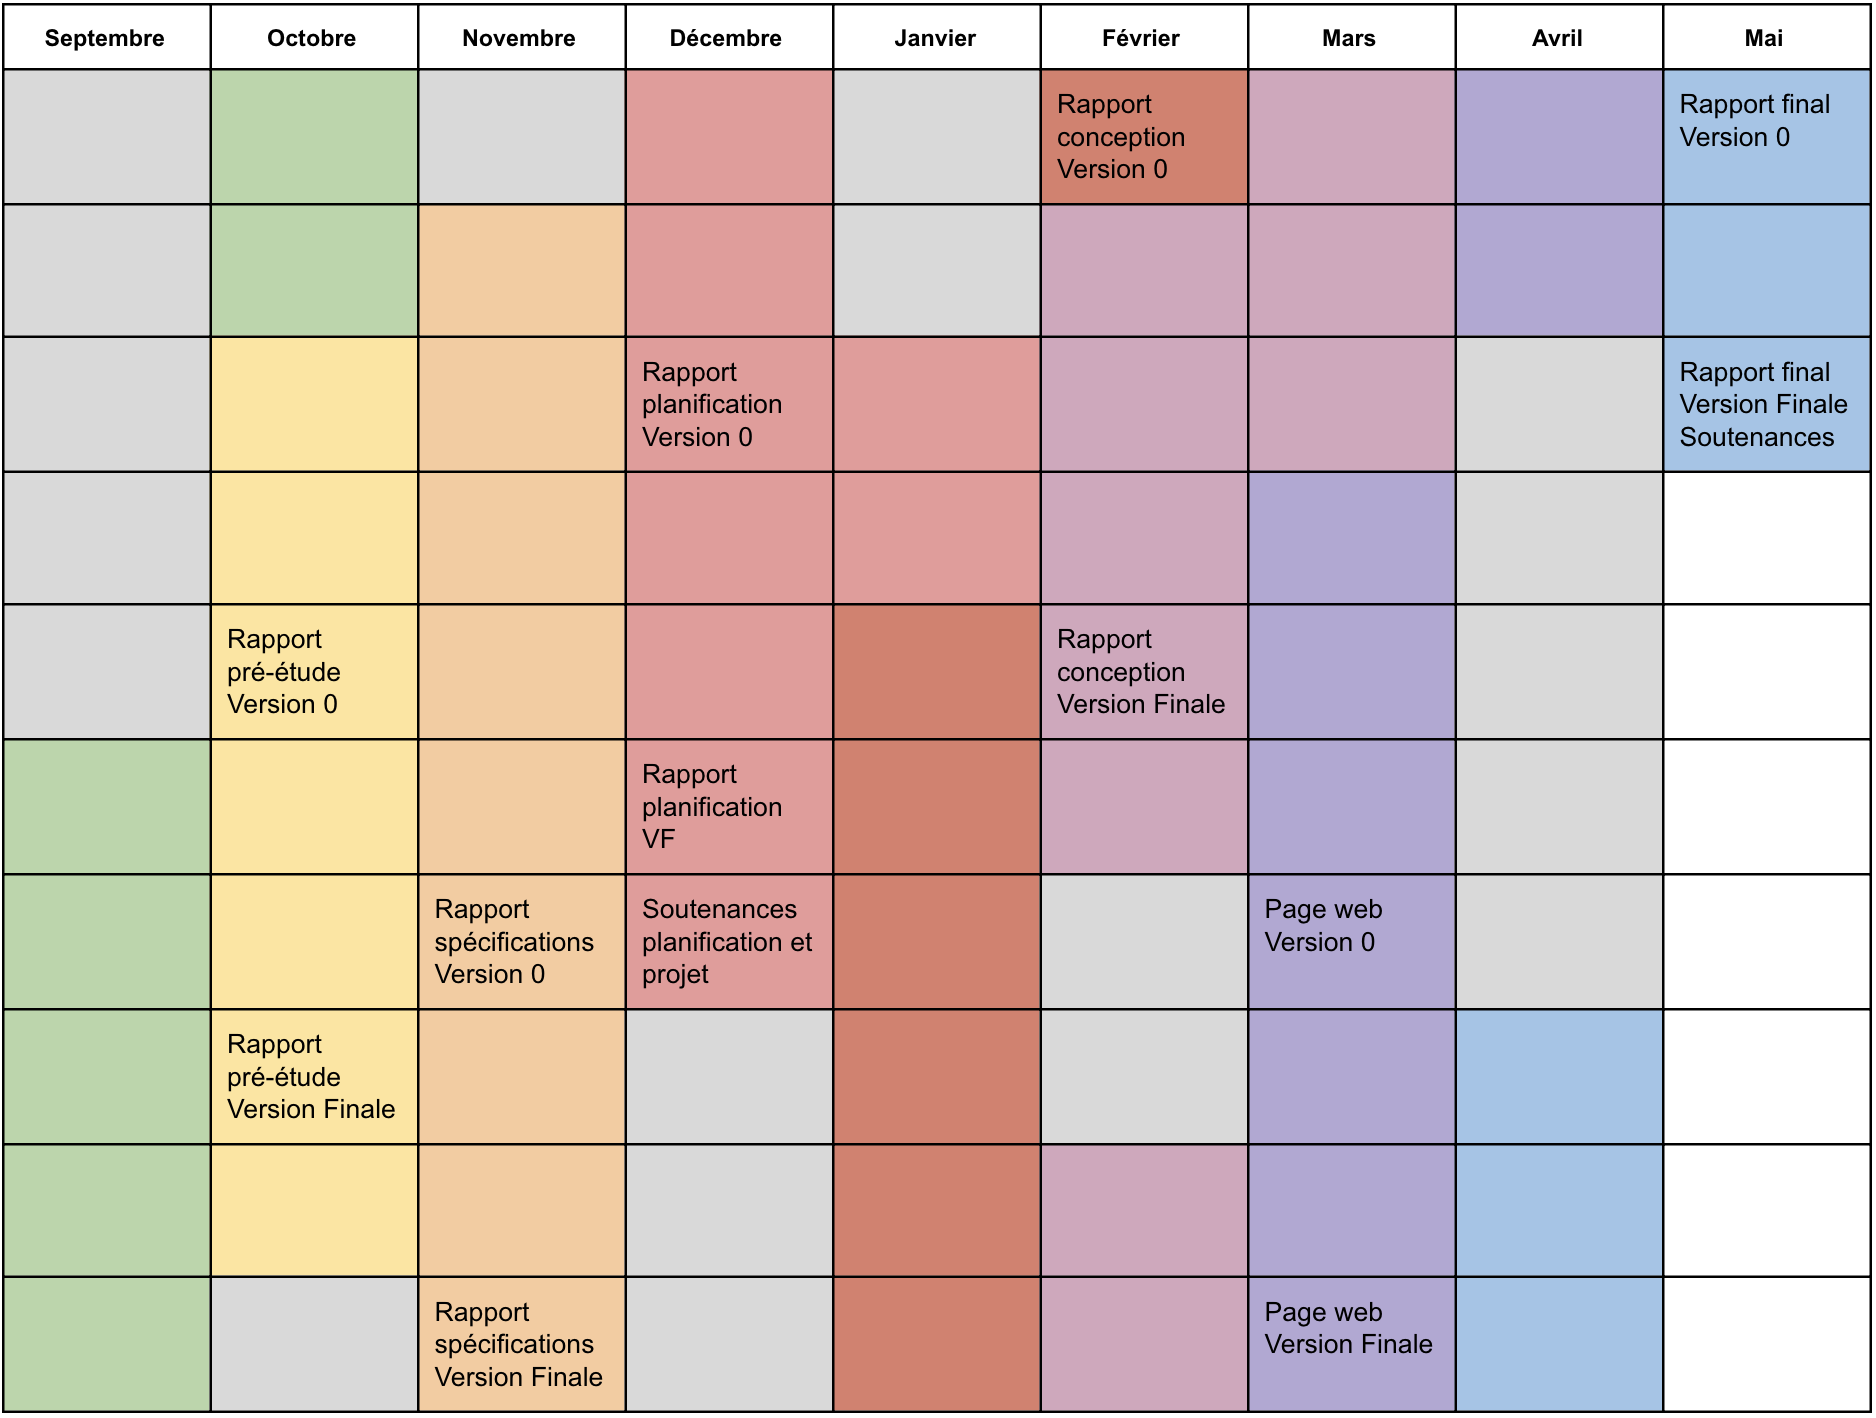
\includegraphics[width=\linewidth]{planning.png}
\end{center}
\end{mdframed}
    
\paragraph{}
Certaines périodes peuvent paraître plus longues pour certains que pour d’autres à cause des vacances
scolaires, mais chacun sera chef de projet durant 3 à 4 semaines. Le rôle du chef de projet est
avant tout de s’assurer du bon déroulement du projet. Il doit organiser les réunions, répartir équitablement
les tâches, surveiller les délais et diriger les réunions. Il doit également faire le lien avec les
différents intervenants et contrôler ce qui est écrit dans les rapports. Le deuxième rôle est celui de
responsable temps qui devra s’assurer que tout le groupe note bien le temps passé sur le projet en envoyant
des rappels réguliers. Il devra également gérer le temps de parole lors des réunions. Pour le moment,
c’est Timothée NEITTHOFFER qui a été désigné responsable temps. La personne jouant ce rôle peut être
modifiée sans problème au cours de l’année. Enfin, le dernier rôle est responsable qualité. Son but est de
contrôler la qualité du code réalisé. Au premier semestre, c’est lui qui valide ou non les technologies que les
autres membres du groupe peuvent lui suggérer en les étudiant. Au second semestre, il devra contrôler le code.
Pour le moment, c’est Enzo CRANCE qui a été désigné responsable qualité. Les autres membres du groupe travaillent
davantage sur les tâches que le chef de projet leur a confié comme la rédaction des rapports, la
recherche d’information, le développement, etc.

\section{Estimation de la planification des tâches}

Pour avoir une première estimation du planning, nous avons construit un diagramme de Gantt en figure 15.

\paragraph{}
\begin{mdframed}[frametitle={Figure 15 : Estimation de la planification des tâches}, innerbottommargin=10]
\begin{center}
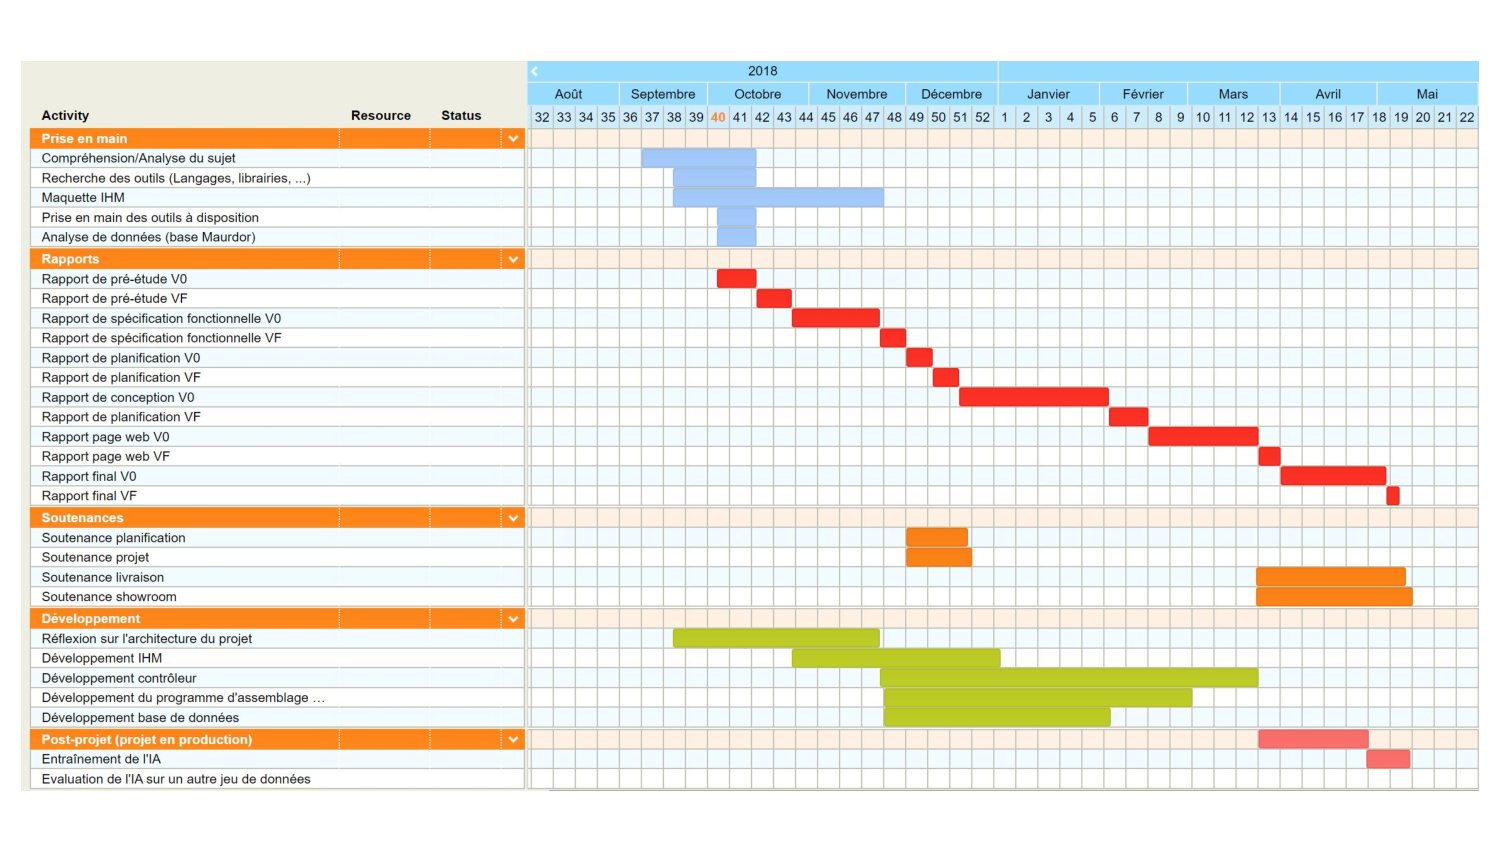
\includegraphics[width=\linewidth]{gantt.pdf}
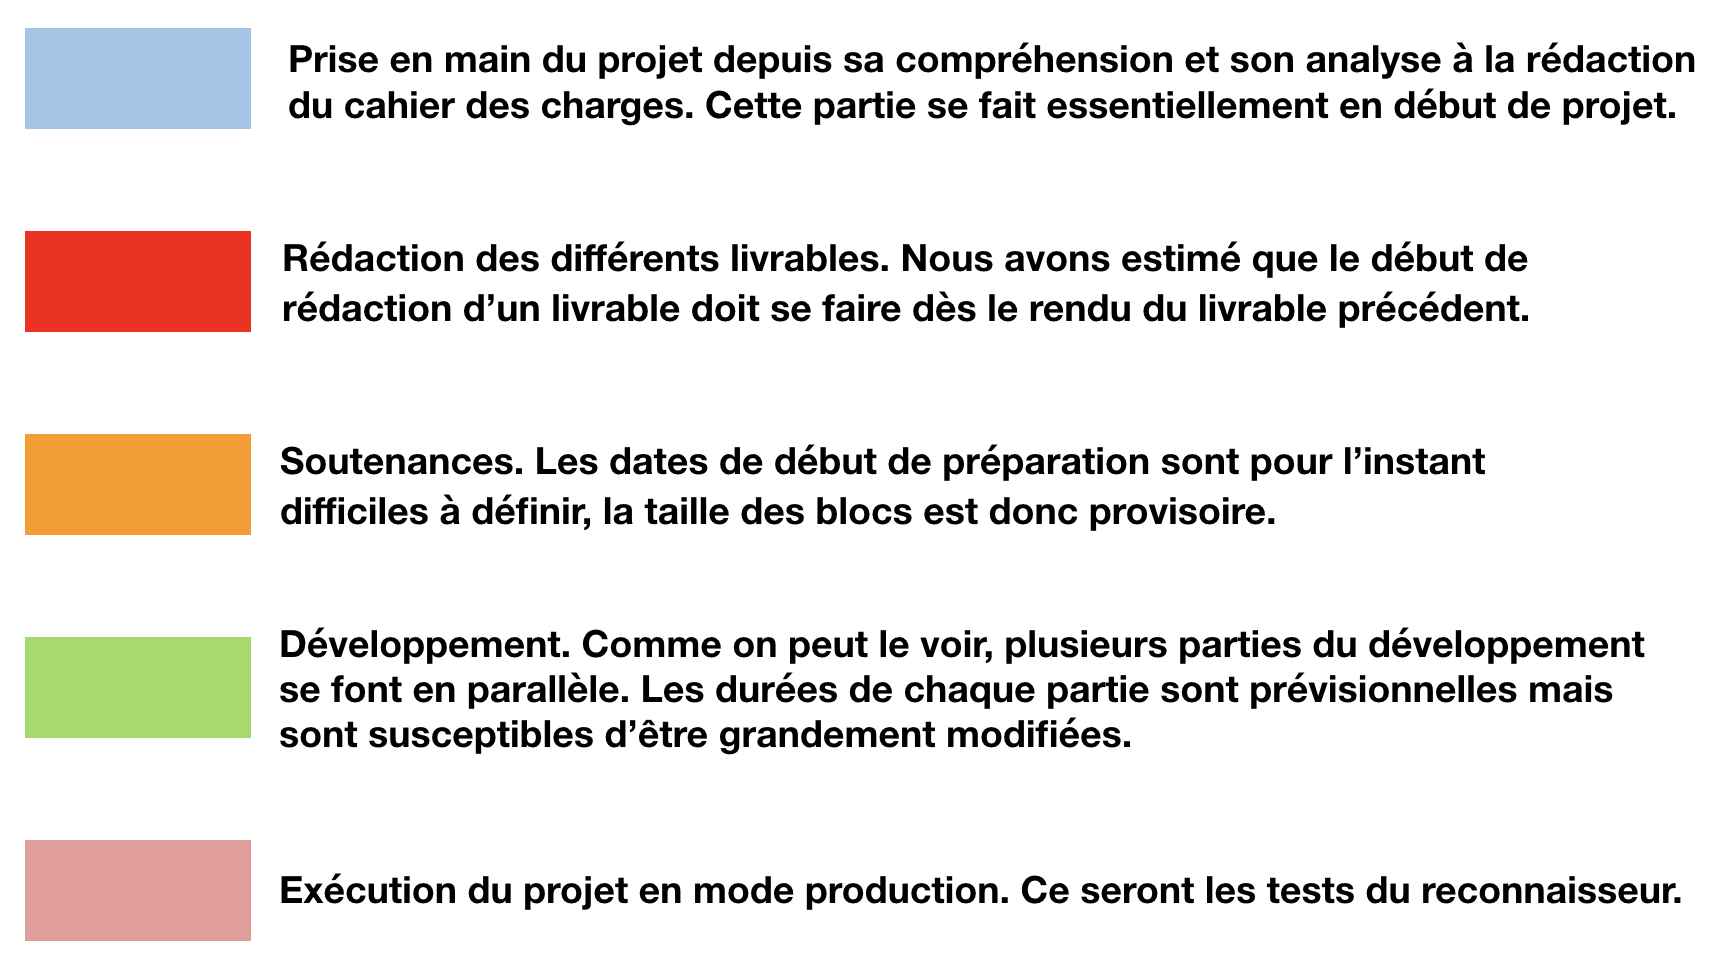
\includegraphics[width=\linewidth]{legende.png}
\end{center}
\end{mdframed}

% ---


\chapter{L'estimation}

\section{Estimation de la partie analyse}

L’estimation des charges de la partie hors développement se résume en deux grands points : le temps passé en réunion ainsi que le temps passé pour la rédaction des rapports et à la préparation des soutenances. Cette partie n’a pas été la plus complexe à estimer car nous avons pu nous baser sur les temps passés lors des trois premiers mois du projet où nous nous sommes concentrés sur la compréhension du cahier des charges et la planification du projet.

\paragraph{}

Pour les deux grands points, le calcul a été sensiblement le même. Dans un premier temps, pour les réunions, nous nous sommes basés sur le temps hebdomadaire passé en réunion depuis le début du projet, au mois de septembre, que nous avons multiplié à la fois par le nombre de semaines restantes et par le nombre de personnes dans le groupe. Dans un  second temps, nous avons calculé le temps nécessaire à la réalisation des prochains rapports. Dans ce cas, nous avons multiplié le temps passé en moyenne par chaque personne pour l’écriture d’un rapport par le nombre de personnes dans le groupe et par le nombre de rapports qu’il nous reste à rendre. Nous avons pu calculer la charge des rapports de cette façon, car nous avons réparti leurs réalisations de façon homogène entre les différents membres du groupe.

\section{Estimation de la partie développement}

Cette partie a été plus compliquée à estimer car nous avions peu de repères. Pour nous rapprocher au maximum d’une estimation fiable, nous avons estimé le temps de développement de chaque partie en considérant les points suivants : 

\begin{itemize}
\item connaissance des technologies utilisées (donc temps d’apprentissage nécessaire estimé) ;
\item temps estimé de conception ;
\item temps estimé de développement .
\end{itemize}

\subsection{Estimation du temps d'apprentissage}

Les différentes technologies qui seront utilisées ont été définies dans le rapport de spécification. Nous savons donc déjà quelles technologies devront être apprises avant de commencer le développement. Le temps d’apprentissage a été défini grossièrement en nous basant sur notre expérience d’auto-formation sur des langages ou d’autres types de technologie.

\newpage

\subsection{Estimation du temps de conception}

La conception ayant majoritairement été réalisée précédemment, cette partie est presque inexistante. Cependant, il est possible que la conception réalisée soit éloignée des réalités techniques. Nous avons donc prévu un temps de remodélisation si nous nous rendons compte à un moment que notre première modélisation n’était pas applicable.

\subsection{Estimation du temps de développement}

Cette partie de l’estimation est la plus compliquée à estimer. En effet, il n’est pas possible de prévoir les problèmes que nous allons rencontrer. C’est pourquoi, nous nous sommes basés sur le temps de développement d’autres projets que nous avons réalisés en y ajoutant une marge au cas où nous serions confrontés à un problème. Afin d’essayer d’obtenir une approximation plus proche de la réalité, nous avons divisé en plus petites parties les objectifs de chacun. Ainsi, alors qu’un grand projet peut paraître vague à estimer, raisonner sur des petites parties concrètes nous permet cette granularité.


% ---


\chapter{Planification : à partir de Microsoft Project}

\section{Hiérarchie des tâches}

Le projet est découpé en 6 tâches principales. Les tâches représentent les différentes
étapes techniques par lesquelles nous devrons passer pour développer le projet.

\begin{itemize}
\item préparation des données ;
\item stockage des données ;
\item interface avec le reconnaisseur ;
\item IHM ;
\item généralités ;
\item écriture des rapports et préparation des soutenances.
\end{itemize}

\paragraph{}

Le projet se déroule de manière parallèle en règle générale, mais chaque bloc a un fonctionnement interne séquentiel, chaque grande tâche est divisée en sous-tâches. Nous avons estimé la durée des différentes tâches d’après notre expérience sur les différents travaux pratiques et projets effectués au cours de notre formation.

\paragraph{}

Tout d’abord, la partie \textbf{préparation des données} consiste à traiter les documents que l’utilisateur souhaite intégrer au logiciel pour pouvoir les découper et les mettre dans un format compatible avec la base de données. Cette partie représente selon notre estimation 77 heures de travail.

\paragraph{}

Ensuite, la partie \textbf{stockage des données} consiste à créer une base de données (choix de la manière de stocker les données établi dans le rapport de spécifications) pour enregistrer les exemples d’apprentissage donnés par l’utilisateur et fournir une interface pour extraire ces données. Cette partie représente environ 10 heures de travail, une grande partie ayant été faite au premier semestre.

\paragraph{}

La partie \textbf{interface avec le reconnaisseur} consiste à fournir une interface entre le stockage et le système de reconnaissance d’écriture manuscrite. Cette partie a été estimée à 40 heures de travail.

\paragraph{}

La partie \textbf{IHM} est la partie fournissant l’interface entre le logiciel et l’utilisateur. C’est dans cette partie que le plus de travail reste à faire, que nous avons estimé à 85 heures.

\paragraph{}

La partie \textbf{généralités} est une partie regroupant des travaux globaux sur le logiciel (lier les blocs entre eux, concevoir un logiciel évolutif, etc. ). Cela représente environ 16 heures de travail.

\paragraph{}

Enfin, les \textbf{rapports et soutenances} représentent une partie non négligeable du travail et surtout la partie la plus contrainte aux dates de rendus. Nous avons estimés cette partie à 63 heures de travail : environ 15 heures par rapport, 10 heures pour la soutenance, et 23 heures pour la page HTML.

\paragraph{}

La durée totale du projet est estimée à 228 heures.

\paragraph{}

\begin{mdframed}[frametitle={Figure 2 : Diagramme de répartition du travail par bloc}, innerbottommargin=10]
\begin{center}
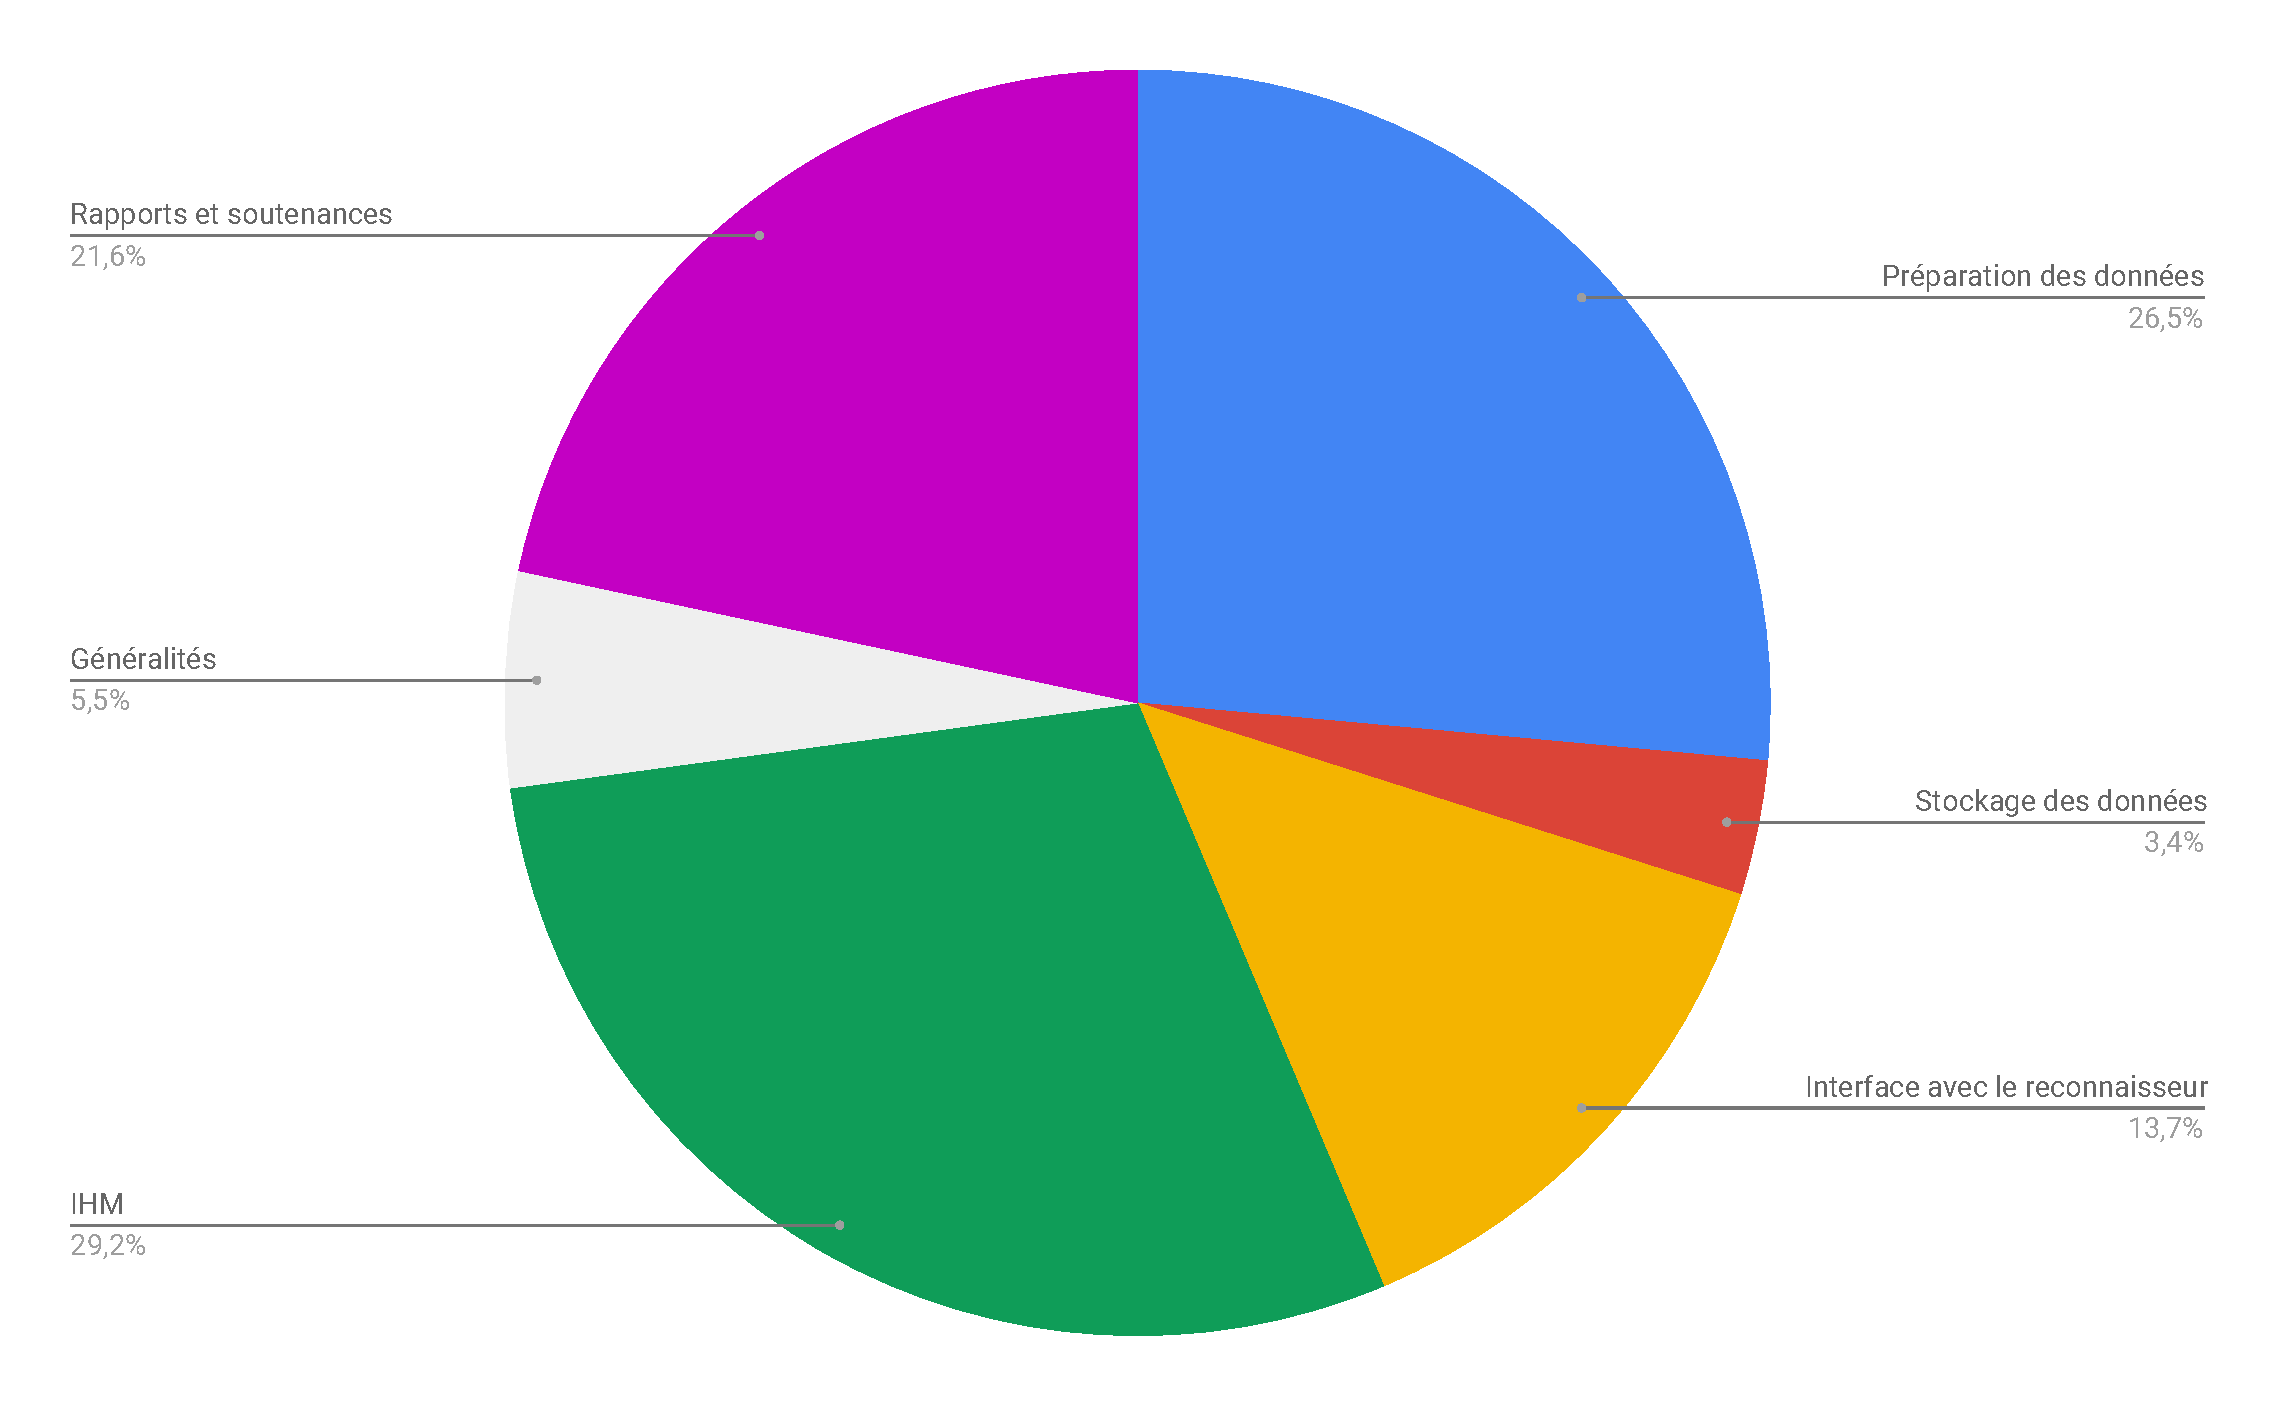
\includegraphics[scale=0.44]{repartition_travail_blocs.pdf}
\end{center}
\end{mdframed}

\section{Affectation des ressources par tâche}

Nous avons fait le choix de spécifier une ressource générique, un membre de l’équipe dans notre cas. Ce choix nous permet de garder une certaine liberté sur l’attribution des tâches durant le développement en nous permettant notamment d’affecter les tâches à un autre développeur à un instant donné. Pour le moment les développeurs ont été répartis sur chacun des blocs mais si certains blocs avancent plus vite que d’autres, il sera possible de réattribuer les rôles. Nous avons essayé de mettre au moins deux personnes par tâche pour que personne ne se retrouve seul face à un problème. Pour les tâches plus simples ou plus rapides nous n'avons mis qu'une seule personne.

\paragraph{}

Ainsi Laure et Charlotte travaillent sur la partie IHM, cette partie étant importante et comprenant suffisamment de travail pour nécessiter deux personnes dessus s’y consacrant entièrement. Timothée travaille sur la partie interface avec le reconnaisseur, cette partie est plus petite que les autres et ne nécessite qu’une personne pour être réalisée. 

\paragraph{}

La partie stockage des données est une partie différente des autres car la base de données a déjà été terminée lors du premier semestre. Ainsi, Timothée et Valentin travailleront dessus au début du second semestre pour vérifier son bon fonctionnement puis Valentin travaillera dessus seul pour terminer l’interface permettant d’y accéder. De même, le développement de la partie préparation des données a été entamé durant le premier semestre. Bien qu’étant une partie importante du projet, elle est déjà bien avancée. De fait, au début du second semestre, Enzo travaillera seul dessus, puis il sera rejoint par Valentin pour l’aider.

\paragraph{}

Concernant la répartition du travail sur les rapports, il a été estimé un travail égal pour chaque personne. Etant donné que les membres de l’équipe sont répartis en blocs, au moins un membre de chaque doit écrire une partie du rapport. Nous sommes donc partis du principe que le travail sur le rapport serait équitablement réparti dans chaque bloc, mais la répartition intra-blocs se fera en réalité au moment de l’écriture entre les membres de l’équipe.

\paragraph{}

Cette répartition permet de répartir la charge de travail de manière équilibrée. Selon notre estimation du temps de travail pour chaque tâche, chaque membre du groupe a une charge de travail égale (entre 42 et 43 heures).

\section{Jalons}

En plus de la planification du temps de développement, nous avons intégré à notre planning des jalons qui correspondent aux dates de rendus et de soutenance. Nous avons attribué l’ensemble des ressources sur les phases de préparation des rendus et des soutenances.

\section{Diagramme de Gantt}

\begin{mdframed}[frametitle={Figure 3 : Diagramme de Gantt du projet (1/2)}, innerbottommargin=10]
\begin{center}
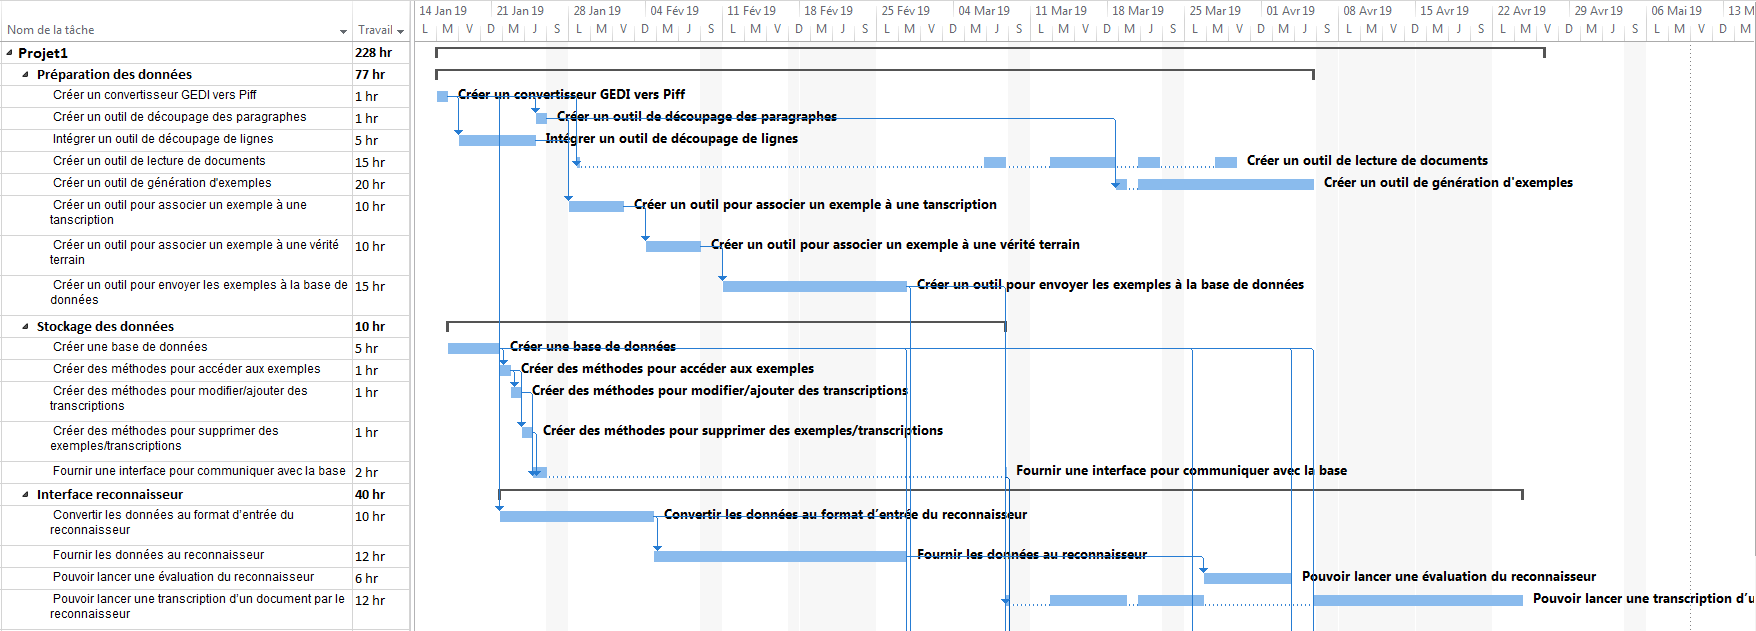
\includegraphics[scale=0.35]{gantt_V2.1.PNG}
\end{center}
\end{mdframed}

\begin{mdframed}[frametitle={Figure 4 : Diagramme de Gantt du projet (2/2)}, innerbottommargin=10]
\begin{center}
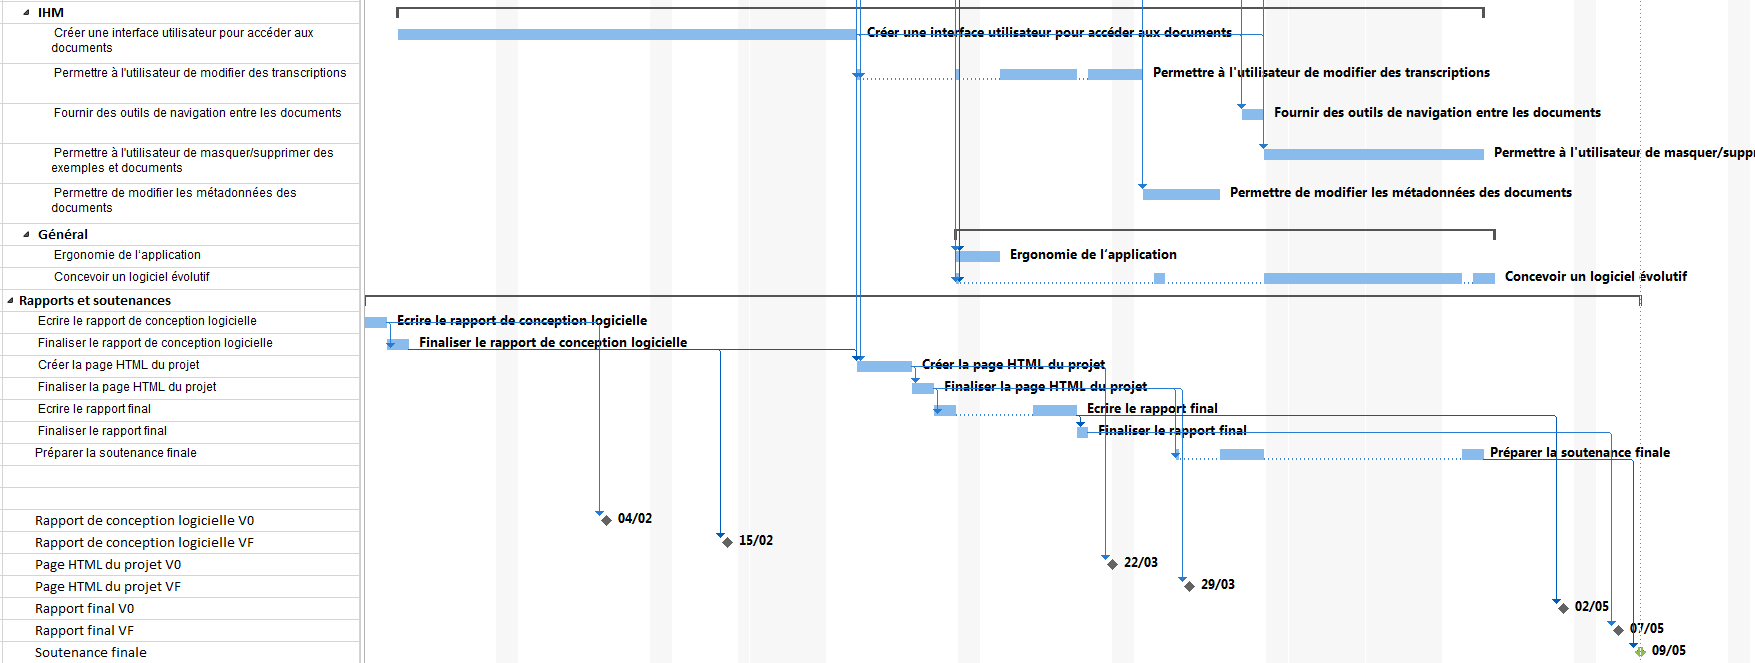
\includegraphics[scale=0.35]{gantt_V2.2.PNG}
\end{center}
\end{mdframed}

Le diagramme de Gantt ci-dessus décrit l’ensemble de la planification du projet, de la conception au rendu final en passant par la gestion de projet ou le développement de chaque itération. On y retrouve également les jalons dont nous avons parlé précédemment.

\newpage

\section{Analyse de la planification}

\subsection{Analyse globale}

Comme dit précédemment, notre projet est constitué de deux itérations. La première itération est constitué des tâches à effectuer avant la création de la page HTML. La seconde est composée des tâches restantes. Comme on peut le voir sur le diagramme, les quatre blocs sont biens parallèles et découpés en tâches. On peut constater que les tâches sont réparties uniformément entre les différents blocs mais que la partie IHM se termine après les autres. Cette partie étant en effet, plus volumineuse, les membres du groupe qui auront terminé leur partie pourront éventuellement aller aider à développer l’IHM en fin  de projet.

\subsection{Tâches critiques}

A partir du diagramme de Gantt, on peut voir apparaître deux tâches critiques, bloquant l’avancement du projet.

\begin{itemize}
\item la création d’un convertisseur GEDI vers Piff est une tâche nécessaire pour l’ensemble des tâches de la préparation de données et de l’interface avec le reconnaisseur ;
\item la création de la base de données est une étape nécessaire pour intégrer la majorité des fonctionnalités de l’IHM .
\end{itemize}

\paragraph{}

Ces tâches doivent être effectuées en priorité pour que le projet puisse avancer. Elles influent en effet sur plusieurs parties du projet. Une fois ces tâches effectuées, la majorité du projet peut se paralléliser. Cet aspect critique a été déduit intuitivement lors de la phase de spécifications du projet, c‘est pourquoi leur développement a été entamé au premier semestre. L’étude avec Microsoft Project a permis de confirmer l’aspect impératif de ces tâches.

\subsection{Ce que l'on peut retenir}

Grâce au diagramme de Gantt, nous avons pu estimer l’organisation de notre travail au second semestre. Selon cette estimation, la date de fin de projet est fixée au vendredi 26 avril. Ce qui nous laisse deux semaines d’avance, avant le dernier rendu. Nous avons également pu confirmer que l’ensemble de notre projet est faisable dans le temps qui nous est imparti. De même, selon Microsoft Project, la réalisation de la première itération pourra être réalisée pour le 27 février. Nous disposerons alors d’une première réalisation fonctionnelle de notre projet, nous aurons du temps pour améliorer cette première version, en collaboration avec le client.
















% ---

\chapter{Conclusion}

Dans le cadre de notre 4\up{ème} année en informatique, nous avons pour mission de
mener à bien un projet de manière plus précise et plus structurée qu’en 3\up{ème} année.
Notre projet, en partenariat avec les archives départementales d’Ille-et-Vilaine,
l’équipe IntuiDoc et Doptim, consiste à créer un logiciel qui aidera les chercheurs et
les ingénieurs à faire progresser la reconnaissance d’écriture manuscrite, afin de rendre
des documents anciens plus accessibles et plus compréhensibles.

\paragraph{}
Notre groupe se compose de 8 étudiants : Enzo CRANCE, Kevin DESPOULAINS, Timothée NEITTHOFFER,
Laure DU MESNILDOT, Charlotte RICHARD, Valentin FOUCHER, Gaël GENDRON et Corentin GUILLOUX.
3 d’entre nous partiront en mobilité internationale au second semestre : Kevin DESPOULAINS,
Gaël GENDRON et Corentin GUILLOUX. Il nous faudra ainsi prendre en compte dans la réalisation
de notre projet ce changement d’effectif. L’étude du projet, la répartition des tâches et la
planification ont donc été faites bien en amont des phases de développement pour permettre à
ceux qui seront encore présents au second semestre de ne pas prendre de retard.

\paragraph{}
Nous avons dans un premier temps étudié ce qui nous était demandé de faire avant de
décider des technologies que nous allions utiliser. Nous avons bien sûr commencé à
étudier les différents outils (langages, API, etc.) que nous pourrions utiliser et qui
feront l’objet du prochain rapport.

\paragraph{}
Nous avons ensuite rédigé notre cahier des charges en reprenant les différentes fonctionnalités
que nous souhaitons développer, en accord avec Bertrand COÜASNON, tout en prenant en compte
les éléments extérieurs avec lesquels notre programme doit communiquer.

\paragraph{}
Nous avons également distribué les rôles qui nous semblent importants pour veiller au bon
déroulement du projet sans mettre trop de pression sur les personnes les endossant.
Un planning prévisionnel a également été rédigé.

%\newpage
%\bibliography{main}
%\bibliographystyle{plain}
%\chapter{Annexes}


\includepdf[pages=-]{pagen.pdf}
\end{document}
